%!TEX root = ../main.tex
%=========================================================

\er{General comments (20220914) after NDSS reject:
\begin{enumerate}
	\item We need to clarify the difference, if any, between \sysname and discv5. Ideally we will want to update the online description which is already several months, if not years, old. I would advocate to present \sysname as the central component of discv5, and detail what are the helping protocols around it (unless, of course, my understanding is incorrect).
	\item Need experiments on prototype.
	\item The use of 100 IPs for the Sybils did not convince one of the two reviewers. Not sure how to fix this?
	\item We should make sure the disctinction between the Ethereum blockchain and the Ethereum ecosystem is clear (confusion with second reviewer).
\end{enumerate}
}
\mk{
Responses to the comments above:
\begin{enumerate}
    \item We consulted it with Felix, at agreed that we can call our think Discv5, while calling the previous one \discv. We should just explain that both Discv5 and \discv have other components (e.g., slightly different encrypted communication) that we don't consider here.
    \item In progress
    \item We'll increase this value in the testbed experiments - it shouldn't influence us that much. 
    \item Yeah, I thought the first part of the introduction was enough, but apparently it wasn't. 
\end{enumerate}
}


\section{Introduction}

With an average of 23,500 constantly live nodes~\cite{discv4-dns-lists}, the Ethereum ecosystem is one of the largest decentralized platforms currently in operation.
While it is widely known for supporting the blockchain of the same name (also known as the \emph{mainnet} and hosted by about 7,000 nodes), the platform is also home to a number of additional decentralized applications.
This includes blockchains used for test purposes (\emph{Ropsten}, \emph{G\"orli}), divergent blockchains resulting from a past fork (\emph{Ethereum classic}), alternative cryptocurrencies (\emph{Pirl}, \emph{Musicoin}), exchange markets (\emph{Binance}), content delivery networks (\emph{Swarm}), or messaging applications (\emph{Whisper}).
The platform already features almost 500 applications, and their number grows every year~\cite{discv4-dns-lists}. The size distribution of the application-specific sub-networks varies significantly (\Cref{fig:ecosystem}) featuring a \emph{long tail}, with a vast majority of applications formed of a few hundred nodes or less.

\begin{figure}[t]
    \includegraphics[width=1\linewidth]{img/ecosystem}
    \vspace{-0.15in}
    \caption{Distribution of the number of nodes of Ethereum's sub-networks in May 2022, corresponding to different applications and sorted by decreasing popularity.
    A Zipf distribution is given for reference.
    }
    \vspace{-0.20in}
    \label{fig:ecosystem}
\end{figure}

All nodes in the Ethereum platform participate in a \emph{global} peer-to-peer (P2P) network operating a distributed hash table (DHT)~\cite{maymounkov2002kademlia}.
In addition to joining the global network, every node connects to at least one \emph{sub-network} formed of peers participating in its application(s) of interest.
In this paper, we focus on the \emph{service discovery} mechanism, by which a node participating in the global P2P network discovers this application sub-network.
Service discovery returns a set of peers that are used as entry points to that sub-network, typically supporting a specific overlay network as illustrated by \Cref{fig:subnetwork}.

\begin{figure}[b!]
    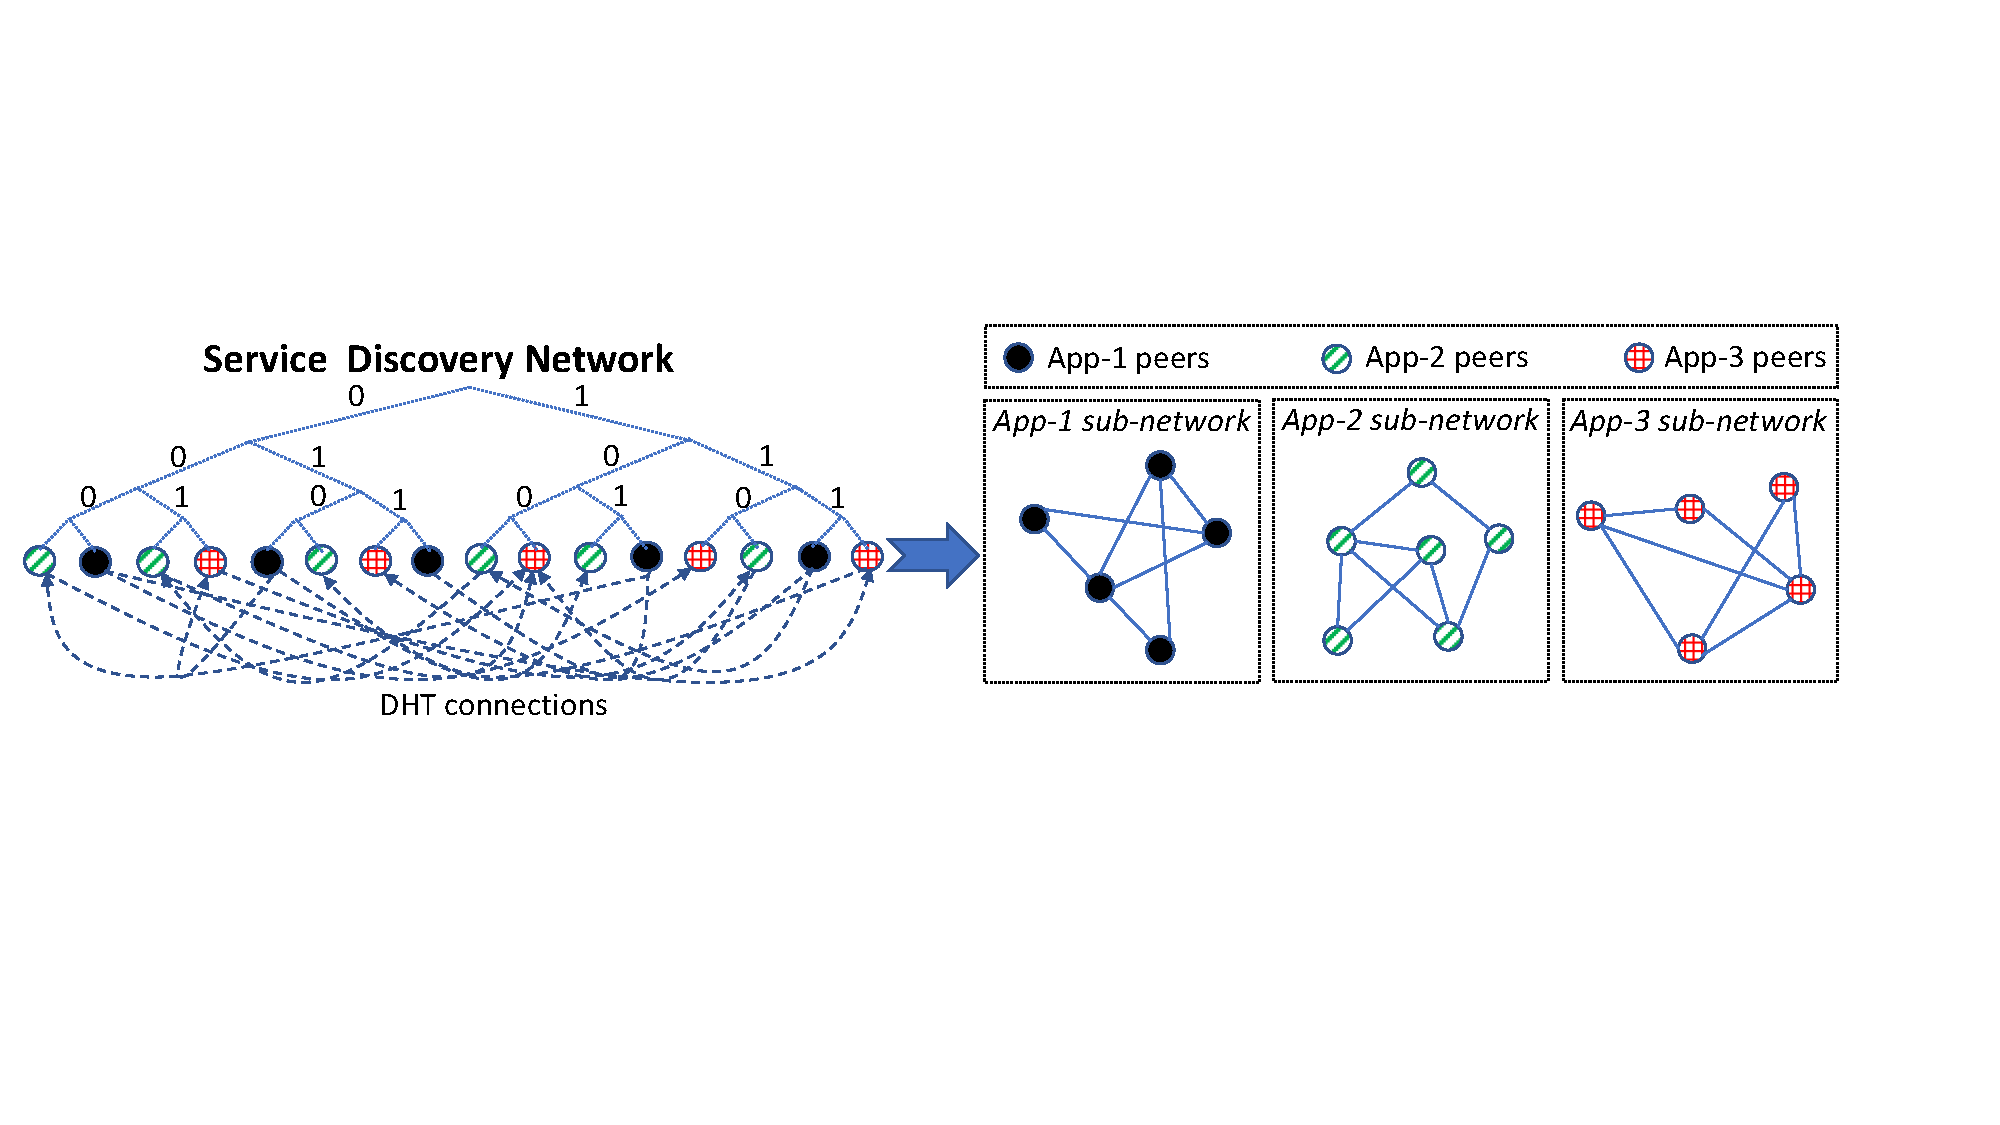
\includegraphics[width=1\linewidth]{img/subnetwork}
    \vspace{-0.15in}
    \caption{Formation of application-specific sub-networks using a universal service discovery network.
    \protect\er{would be good to have larger fonts in the figure, they are very small compared to those of Figure~\ref{fig:ecosystem}}
    }
    \label{fig:subnetwork}
    \vspace{-0.15in}
\end{figure}

Service discovery is a particularly sensitive mechanism in the Ethereum platform.
It must ensure that malicious participants to this open network are unable to bias its execution against a victim node or sub-network--and that, despite the ability of these adversaries to operate multiple Sybil identities.
Of particular importance is the protection against \emph{eclipse} attacks, where an adversary would lure its victim(s) into a sub-network formed of only nodes under its control.
Similarly, an adversary may run \emph{denial-of-service} attacks against a specific application, preventing other nodes from discovering peers from the associated sub-network.
On the other hand, the mechanism must remain efficient and scalable.
It is not desirable, for scalability and robustness reasons, that it relies solely on fixed (sets of) dedicated registrar nodes maintaining the membership of each application.
Registrar nodes for popular applications could quickly become overwhelmed, and they would be an easy target for attackers.
In addition, the need to provision dedicated registrar nodes would be a hindrance to the emergence of new applications and (initially) small sub-networks.

% \er{There are inconsistencies with the presentation of discv4; here presented as a set of protocols but later as the name of the discovery mechanism itself. In general, we should clarify what are these other protocols. If these are helping/lower level protocols for the discovery mechanism I would prefer to present discv4 as the discovery mechanism (and do the same for discv5=\sysname).}
% \mk{Yes, we can to that (see the comments before the intro}

The current service discovery mechanism used in the Ethereum platform, named \discv~\cite{discv4}, leverages the global DHT for service discovery using a simple but robust \emph{random walk} approach.
A node willing to join an application's sub-network simply contacts individually a series of nodes collected from random lookups on the DHT, repeatedly checking application membership until it has collected enough peers participating in this target application.
This approach offers good resilience to malicious behaviors but it suffers from very poor scalability and performance, in particular for small sub-networks.
Random walks have, indeed, a decreasing likelihood of encountering peers from the target sub-network, increasing the number of messages required, join latency, and resource consumption at all the encountered peers.
Our observations of \discv show that it can require no less than \hl{\textbf{XXX}} \er{FILL ME} attempts for a node to find \hl{\textbf{Y}} \er{FILL ME} different peers, for a medium-size sub-network already featuring \textbf{100} nodes, and significantly more for smaller sub-networks.
As more applications join the DHT, the inefficiency of the random discovery process becomes a bottleneck for the entire ecosystem.
While alternative solutions for service discovery have been proposed, they are meant for small-scale network~\cite{zhang2002aggregate, helal2002standards}, centralised~\cite{RFC6763}, based on unrealistic assumptions~\cite{danezis2005sybil, danezis2009sybilinfer}, or insecure~\cite{baldoni2007tera,scribe,poldercast,banno2015,scribe}.
We provide an extensive analysis of these systems in \Cref{sec:related}.

\smallskip
\noindent
\textbf{Contributions.}
%
We present in this paper \sysname, a novel service discovery mechanism for large-scale, decentralized platforms and its application to Ethereum.
\sysname targets a balance between robustness, i.e., the ability to resist malicious behaviors and Sybil identities, efficiency, i.e., fast service discovery even for small applications, and good load-balance over participating nodes.

After providing background knowledge and reviewing the current service discovery mechanism of Ethereum in \Cref{sec:background}, and detailing our system and threat models in \Cref{sec:model}, we detail \sysname as follows.

In \Cref{sec:placement}, we present how this new protocol enables nodes, members of application sub-networks, to \emph{advertise} their membership to these applications in the form of \emph{service advertisements}.
Any node can act as a \emph{registrar} and store advertisements for any topic.
In contrast with the direct use of the DHT as a key-value store, however, in \sysname service advertisements propagate to a pseudo-random subset of all nodes in the global network.
The density of advertisements for an application increases as a DHT lookup approaches its associated key in the DHT overlay structure.

Robustness, load balancing, and efficiency for the discovery of smaller sub-networks all rely on a novel \emph{admission protocol}, by which registrars accept or reject incoming service advertisements (\Cref{sec:admission}).
It ensures that advertisers cannot effectively flood advertisements at a registrar, even when deviating from the protocol or operating Sybils, and that less popular topics get a sufficiently high probability to be represented and looked up. \er{and looked up $\rightarrow$ and found?}

At the core of our novel admission protocol lies the need for registrants to respect a waiting time imposed by the registrars before being able to successfully register their advertisement.
We discuss the design and dynamics of the waiting function in \Cref{sec:waitingTime}.
The function allows limiting the amount of resources used by each node, promotes diversity of topic advertisements stored by each node, and protects against a vast range of malicious behaviors.

% \er{The relation between discv5 and \sysname is unclear. If discv5 is a set of protocols as written below we should detail what the other protocols are. From the webpage description it seems more that the discovery mechanism is the central protocol and other protocols are helper/subsidiary protocols, e.g., for defining the communication standards between nodes in the p2p operation. We should make it clearer that \sysname is the core component of discv5 (or even consider using discv5 name directly if possible, and mention that the other protocols are helpers, if the reasoning above applies).}
% \er{comment is now addressed}

\er{revise this paragraph in light of the deployment results; highlights could focus on real deployments.}
We overcome multiple practical challenges, implement \sysname in a simulator as well as in the code base of \emph{discv5}~\cite{discv5} \er{change me: the code base of Ethereum (two clients right?)} (\ie, Node Discovery protocol version 5) - a new set of P2P protocols replacing \emph{discv4}~\cite{discv4}. 
%We intend to release the full code and dataset of our experiment open source with the unblinded version of this paper.
Compared to the \discv, \sysname discovers 10 times more peers on average by sending two times less lookup messages and achieves a similar or better resistance against eclipse attacks. 
Compared to vanilla DHT operations, our system reduces load on the most busy node in the network by 2 orders of magnitude and is up to 4 orders of magnitude less likely to be eclipsed by a powerful attacker. \er{the metric for the ``eclipsability'' here is not clear. What does it mean to be 4 OOM less likely to be eclipsed?} \mk{In the analysis we calculate what's the probability of an operation returning only malicious results} \er{ok, keeping for now}
\sysname is currently under testnet evaluation and is scheduled for deployment in the future versions of Ethereum network. \er{revise previous if the deployment is actually planned.}
